\documentclass{article}
\usepackage[utf8]{inputenc}
\usepackage{listings}
\usepackage{xcolor}
\usepackage{graphicx}
\graphicspath{ {./Image/} }
\usepackage{caption}
\usepackage{subcaption}
\usepackage{float} 
\usepackage{wrapfig}\usepackage{fancyhdr}

\pagestyle{fancy}
\fancyhf{}
\rhead{Jeppe Matzen}
\lhead{20/10-2020}
\rfoot{Page \thepage}


\definecolor{codegreen}{rgb}{0,0.6,0}
\definecolor{codegray}{rgb}{0.5,0.5,0.5}
\definecolor{codepurple}{rgb}{0.58,0,0.82}
\definecolor{backcolour}{rgb}{0.95,0.95,0.92}

\lstdefinestyle{mystyle}{
    backgroundcolor=\color{backcolour},   
    commentstyle=\color{codegreen},
    keywordstyle=\color{magenta},
    numberstyle=\tiny\color{codegray},
    stringstyle=\color{codepurple},
    basicstyle=\ttfamily\footnotesize,
    breakatwhitespace=false,         
    breaklines=true,                 
    captionpos=b,                    
    keepspaces=true,                 
    numbers=left,                    
    numbersep=5pt,                  
    showspaces=false,                
    showstringspaces=false,
    showtabs=false,                  
    tabsize=4
}

\title{Mini Project 2: Morphological operations}
\author{Jeppe Matzen}
\date{September 2020}



\begin{document}

\lstset{style=mystyle}
\maketitle

\section{Aim:}
Målet med mini projekt 2, Morphological operations, er at overfører teori til $C++$ kode ved at anvende funktionerne på virkelige medicinske billeder. \newline 
For selv at kunne konstruere $C++$ funktioner fra bunden og anvende dem er det nødvendigt at forstå formålet og fremgangsmåden til mindste detalje.  

\section{Discussion:}

\subsection{Opgave 1:}
I opgave 1 bruges morphological operations til at behandle billedet. Målet med disse operationer er at fjerne uønskede elementer og fremhæve ønskede på binære billeder. \newline
En af de operationer der benyttes er erosion. Erosion fjerner et lag af pixels rundt om strukturer. Dette resultere i at mellemrummet mellem eller huller i strukture bliver større. Erosion resultere i at de små detailjer i billedet fjernes.\newline
Dilation er det modsatte af erosion. Dilation tilføjer et lag rundt om strukturer. Dette resultere i at mellemrummet mellem strukturer bliver mindre og eventuelle huller bliver udfyldt. \newline
Inden erosion og dilation kan blive brugt skal billedet thresholdes. Til dette blev Otsu thredshold brugt.
Otsu thredshold opdeler billedets pixels i to grupper og finder den thredshold værdi der giver den mindste gruppe variance og den største variance mellem grupper.  

\subsection{Opgave 2:}
For at udregne forholdet mellem algoritmens optegning af blodåre og de faktiske
blodåre, blev antallet af pixels, med værdien 255, i resultat billedet talt.
Herefter blev værdien af hver enkel pixel, for hver position, sammenliget for de to billeder. Hvis de var lig med hinanden, og lig 255, blev værdien af grønne pixels talt en op. Til slut kunne forholdet findes ved at dividere antallet af grønne pixles med antallet af røde pixels. 

\subsection{Opgave 3:}
Adabted thredshold

Connected Compontents:



\section{Results:}
\subsection{Opgave 1:}
For at løse opgave to skulle billedet først thredsholdes. Det blev gjort ved at kigge på histogrammet for billedet. Ud fra histogrammet vurderes det hvilken thredshold metode der er den bedste i denne situation. Da histogrammet for billedet \ref{fig:f3} har en binormal fordeling er Otsu thredshold den bedste metode.\newline
På \ref{fig:f4} er alle rice markeret. De er markeret ved en erosion. En erosion vil markere den yderste kant af alle rice kornene. Hvis der var blevet brugt dilation, ville der være blevet markeret rundt om alle rice kornene. Dette ville kunne have resulteret i at nogle rice strukturer flød sammen, og dette ville give et resultat der er forskelligt fra virkeligheden.  
\begin{figure}[!h]
	\begin{subfigure}[b]{0.49\linewidth}
		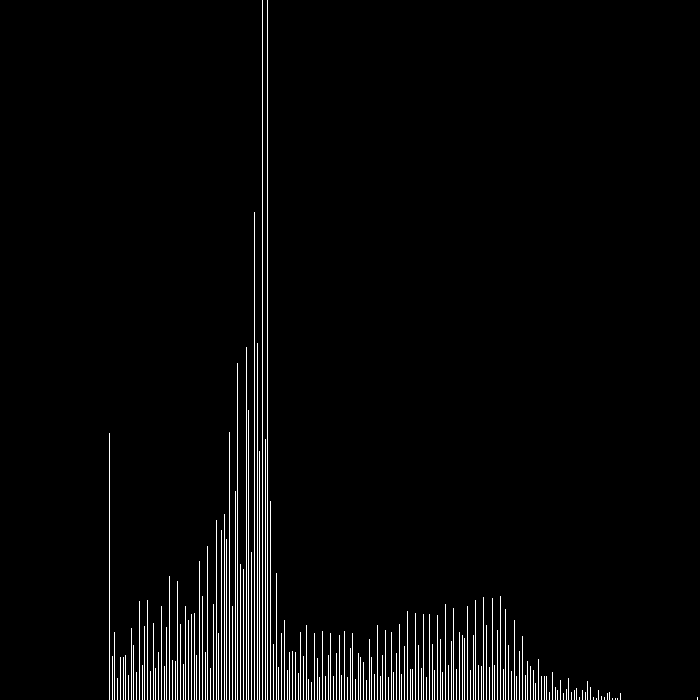
\includegraphics[width=\linewidth]{histogram.png}
		\caption{Thredsholded billede af Rice}
		\label{fig:f3}
	\end{subfigure}
	\hfill
	\begin{subfigure}[b]{0.49\linewidth}
		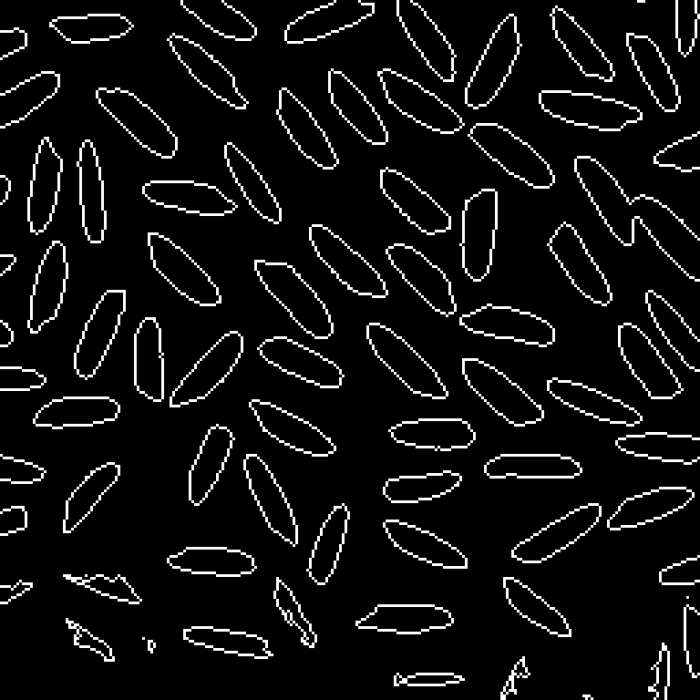
\includegraphics[width=\linewidth]{cornOutlined.png}
		\caption{Grænsen af Rice markedet}
		\label{fig:f4}
	\end{subfigure}
	\caption{}
	\label{fig:image2}
\end{figure}

\subsection{Opgave 2:}
Figur \ref{fig:f2} viser det område hvor algoritmen og virkeligheden stemmer overens. 
Forholdet mellem de røde pixels og de grønne pixels er: $$\frac{4378}{12137} = 0.360715$$
\begin{figure}[!h]
	\begin{subfigure}[b]{0.49\linewidth}
		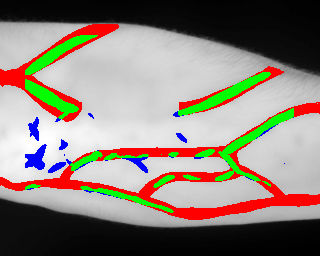
\includegraphics[width=\linewidth]{RoBlood_result.png}
		\caption{Billede af lunge.}
		\label{fig:f1}
	\end{subfigure}
	\hfill
	\begin{subfigure}[b]{0.49\linewidth}
		
\includegraphics[width=\linewidth]{greenPixels.png}
		\caption{Histogram af lunge billede}
		\label{fig:f2}
	\end{subfigure}
	\caption{}
	\label{fig:image1}
\end{figure}

\subsection{Opgave 3:}

\end{document}
